\documentclass[11pt,a4paper]{article}
\usepackage[utf8]{inputenc}
\usepackage[T1]{fontenc}
\renewcommand{\contentsname}{Índice}\renewcommand{\figurename}{Figura}\renewcommand{\tablename}{Tabela}
\usepackage[margin=2.5cm]{geometry}
\usepackage{amsmath,amssymb,amsthm}
\usepackage{booktabs}
\usepackage{listings}
\usepackage{xcolor}
\usepackage{tikz}
\usetikzlibrary{arrows.meta,calc}
\usepackage[hidelinks]{hyperref}
\usepackage{enumitem}
\usepackage{float}

\setlength{\parskip}{0.5em}
\setlength{\parindent}{0pt}

\lstset{basicstyle=\ttfamily\small,breaklines=true,frame=single,columns=fullflexible,
  keywordstyle=\color{blue!60!black},commentstyle=\color{green!40!black},
  language=C++,showstringspaces=false}

% ---------- notacao ----------
\newcommand{\vv}[1]{\mathbf{#1}}              % vetor
\newcommand{\col}[3]{\begin{pmatrix}#1\\#2\\#3\end{pmatrix}}
\newcommand{\cs}{\cos}
\newcommand{\sn}{\sin}
\newcommand{\Rot}{\mathbf{R}}
\newcommand{\Id}{\mathbf{I}}
\newcommand{\T}{^{\mathsf{T}}}

\theoremstyle{definition}
\newtheorem{deducao}{Dedução}[section]
\newtheorem{exemplo}{Exemplo}[section]
\newcommand{\resultado}[1]{\begin{center}\fbox{\parbox{0.9\textwidth}{\centering #1}}\end{center}}

\title{\textbf{Visualizador 3D de Trajetórias de Robôs Subaquáticos}\\[0.3em]
\large Fundamentos matemáticos, referenciais e vista em 1.ª pessoa}
\author{Documentação das bibliotecas matemáticas (C++ OOP) e da aplicação (Python)}
\date{1 de outubro de 2026}

\begin{document}
\maketitle
\tableofcontents
\newpage

%=====================================================================
\section{Introdução e convenções}
%=====================================================================
Este documento explica a matemática usada pelo visualizador 3D de trajetórias e pela vista em 1.ª pessoa (o ponto de vista de cada drone). Cada fórmula é \emph{deduzida passo a passo} a partir de definições simples, sem saltar contas.

\subsection{Arquitetura em duas linguagens}
\begin{itemize}[nosep]
  \item \textbf{Python}: aplicação, leitura de configuração, interface e visualização.
  \item \textbf{C++ (orientado a objetos)}: toda a matemática (vetores, matrizes, rotações, referenciais, geodesia, câmara). É uma biblioteca reutilizável, chamada a partir do Python.
\end{itemize}

\subsection{Regras de notação}
Para que tudo seja fácil de acompanhar, usa-se sempre a mesma notação:
\begin{itemize}[nosep]
  \item Posições e vetores são \textbf{vetores coluna} de 3 componentes, escritos com $x$, $y$, $z$:
  $\vv{p}=\col{x}{y}{z}$.
  \item Todas as matrizes são de dimensão $3\times 3$ (\textbf{não} se usam matrizes homogéneas $4\times 4$). Uma mudança de referencial escreve-se com uma matriz $3\times3$ \emph{mais} um vetor de translação, de forma explícita.
  \item Ângulos em radianos. $\cs$ e $\sn$ abreviam-se por $c$ e $s$ nas matrizes grandes, com o ângulo no índice: $c_\psi=\cos\psi$.
  \item O índice inferior indica o referencial em que um vetor está escrito: $\vv{p}_w$ (mundo), $\vv{p}_b$ (corpo do drone), $\vv{p}_c$ (câmara).
  \item $\Rot_{wb}$ é a matriz que converte \emph{do referencial b para o referencial w}. Lê-se da direita para a esquerda: $\vv{p}_w=\Rot_{wb}\,\vv{p}_b+\ldots$
\end{itemize}

\begin{table}[H]
\centering
\begin{tabular}{ll}
\toprule
Símbolo & Significado\\
\midrule
$\vv{p}_w=(x,y,z)\T$ & posição no referencial do mundo (NED)\\
$\vv{t}_{wb}$ & posição da origem do corpo b, escrita em w\\
$\Rot_{wb}$ & matriz $3\times3$ de rotação de b para w\\
$\phi,\theta,\psi$ & roll (rolamento), pitch (arfagem), yaw (guinada)\\
$\vv{v}$, $\vv{\omega}$ & velocidade linear, velocidade angular\\
$f_x,f_y,c_x,c_y$ & parâmetros da câmara (distância focal e ponto principal)\\
\bottomrule
\end{tabular}
\caption{Símbolos usados no documento.}
\end{table}

%=====================================================================
\section{Referenciais}
%=====================================================================
Um \emph{referencial} é uma origem mais três eixos perpendiculares entre si. Usam-se quatro:

\begin{enumerate}
  \item \textbf{ECEF} (Earth-Centered, Earth-Fixed): origem no centro da Terra, $z$ pelo eixo de rotação (Polo Norte), $x$ no cruzamento do equador com o meridiano de Greenwich, $y$ completa o sistema direito. Serve para coordenadas globais (GPS).
  \item \textbf{NED} (North--East--Down): referencial local do mundo, com origem num ponto de referência. $x$ aponta para Norte, $y$ para Este, $z$ para baixo. É o usado na simulação. Como $z$ cresce para baixo, \textbf{a profundidade de um robô subaquático é diretamente a sua coordenada $z$}.
  \item \textbf{Corpo} (b): preso ao drone. $x_b$ para a frente, $y_b$ para a direita, $z_b$ para baixo.
  \item \textbf{Câmara} (c): preso à câmara do drone. $x_c$ para a direita da imagem, $y_c$ para baixo da imagem, $z_c$ para a frente (eixo ótico).
\end{enumerate}

Todos são sistemas \textbf{direitos}: $\hat{x}\times\hat{y}=\hat{z}$.

\begin{figure}[H]
\centering
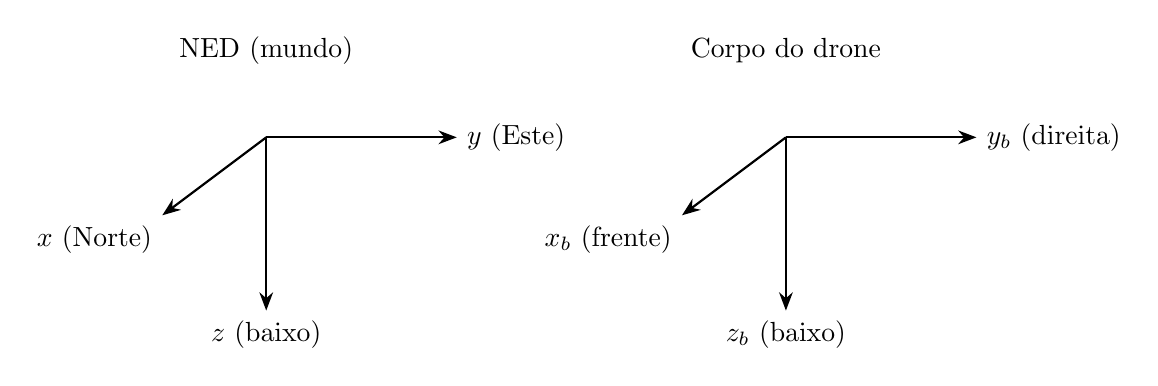
\begin{tikzpicture}[scale=1.1,>=Stealth]
  % NED
  \begin{scope}
    \draw[->,thick] (0,0) -- (2.2,0.0) node[right] {$y$ (Este)};
    \draw[->,thick] (0,0) -- (-1.2,-0.9) node[below left] {$x$ (Norte)};
    \draw[->,thick] (0,0) -- (0,-2.0) node[below] {$z$ (baixo)};
    \node at (0,1.0) {NED (mundo)};
  \end{scope}
  % corpo
  \begin{scope}[xshift=6cm]
    \draw[->,thick] (0,0) -- (-1.2,-0.9) node[below left] {$x_b$ (frente)};
    \draw[->,thick] (0,0) -- (2.2,0.0) node[right] {$y_b$ (direita)};
    \draw[->,thick] (0,0) -- (0,-2.0) node[below] {$z_b$ (baixo)};
    \node at (0,1.0) {Corpo do drone};
  \end{scope}
\end{tikzpicture}
\caption{Os eixos do mundo (NED) e do corpo têm a mesma disposição; só diferem na origem e na orientação (que o drone pode rodar).}
\end{figure}

%=====================================================================
\section{Geodesia: de latitude/longitude para coordenadas locais}
%=====================================================================
Quando os dados chegam como latitude $\varphi$, longitude $\lambda$ e altura $h$ (GPS), é preciso convertê-los para o referencial NED.

\subsection{Latitude, longitude, altura $\rightarrow$ ECEF}

A Terra é modelada por um elipsoide (WGS84) com semieixo maior $a$ (equador) e semieixo menor $b$ (polos). A excentricidade $e$ define-se por
\begin{equation}
e^2 = 1-\frac{b^2}{a^2}\quad\Longrightarrow\quad b^2=a^2(1-e^2).
\label{eq:e2}
\end{equation}

\begin{deducao}[Coordenadas ECEF de um ponto na superfície]
\textbf{Passo 1 --- Elipse do meridiano.} Cortando o elipsoide por um plano que contém o eixo $z$, obtém-se uma elipse. Chamamos $\rho$ à distância ao eixo $z$ (no plano do equador) e $z$ à altura. A elipse é
\[
\frac{\rho^2}{a^2}+\frac{z^2}{b^2}=1 .
\]

\textbf{Passo 2 --- Declive da normal.} A latitude geodésica $\varphi$ é o ângulo entre a normal à superfície e o plano do equador. Derivando implicitamente a elipse:
\[
\frac{2\rho}{a^2}+\frac{2z}{b^2}\frac{dz}{d\rho}=0
\;\Longrightarrow\;
\frac{dz}{d\rho}=-\frac{b^2\rho}{a^2 z}.
\]
Este é o declive da tangente. A normal é perpendicular, logo o seu declive é o simétrico do inverso:
\[
\tan\varphi=\frac{a^2 z}{b^2\rho}\;\Longrightarrow\; z=\frac{b^2}{a^2}\,\rho\tan\varphi=(1-e^2)\,\rho\tan\varphi,
\]
onde se usou \eqref{eq:e2}.

\textbf{Passo 3 --- Substituir na elipse.} Metendo $z$ na equação da elipse e usando $b^2=a^2(1-e^2)$:
\[
\frac{\rho^2}{a^2}+\frac{(1-e^2)^2\rho^2\tan^2\varphi}{a^2(1-e^2)}=1
\;\Longrightarrow\;
\frac{\rho^2}{a^2}\Big[1+(1-e^2)\tan^2\varphi\Big]=1 .
\]

\textbf{Passo 4 --- Resolver em $\rho$.} Multiplicando o parêntesis por $\cos^2\varphi$ em cima e em baixo:
\[
\rho^2=\frac{a^2\cos^2\varphi}{\cos^2\varphi+(1-e^2)\sin^2\varphi}
=\frac{a^2\cos^2\varphi}{1-e^2\sin^2\varphi},
\]
pois $\cos^2\varphi+\sin^2\varphi=1$. Definindo
\begin{equation}
N=\frac{a}{\sqrt{1-e^2\sin^2\varphi}},
\label{eq:N}
\end{equation}
fica $\rho=N\cos\varphi$ e, do passo 2, $z=(1-e^2)\,N\cos\varphi\tan\varphi=N(1-e^2)\sin\varphi$.

\textbf{Passo 5 --- Rodar para a longitude.} O ponto está no plano do meridiano; rodar em torno de $z$ pelo ângulo $\lambda$ dá $x=\rho\cos\lambda$, $y=\rho\sin\lambda$.

\textbf{Passo 6 --- Acrescentar a altura $h$.} Subir $h$ ao longo da normal, cuja direção unitária é $(\cos\varphi\cos\lambda,\;\cos\varphi\sin\lambda,\;\sin\varphi)\T$ (ver Dedução~\ref{ded:vetores}).
\end{deducao}

\resultado{$\displaystyle
\col{X}{Y}{Z}_{\text{ECEF}}=
\col{(N+h)\cos\varphi\cos\lambda}{(N+h)\cos\varphi\sin\lambda}{\big(N(1-e^2)+h\big)\sin\varphi}$,\quad
$N=\dfrac{a}{\sqrt{1-e^2\sin^2\varphi}}$}

Para um robô subaquático, $h$ é negativo (abaixo do nível do mar): $h=-\text{profundidade}$.

\subsection{ECEF $\rightarrow$ NED}

\begin{deducao}[Eixos locais Norte, Este, Baixo em ECEF]\label{ded:vetores}
Seja $\vv{r}(\varphi,\lambda)$ a posição ECEF de um ponto à superfície (com $h=0$). As direções locais obtêm-se derivando $\vv{r}$ e normalizando.

\textbf{Este} é a direção em que só $\lambda$ aumenta:
\[
\frac{\partial\vv{r}}{\partial\lambda}=\col{-\rho\sin\lambda}{\rho\cos\lambda}{0}
\;\Longrightarrow\;
\hat{e}=\col{-\sin\lambda}{\cos\lambda}{0}
\]
(divide-se pelo comprimento $\rho$).

\textbf{Norte} é a direção em que só $\varphi$ aumenta. Derivando $\rho=N\cos\varphi$ e $z=N(1-e^2)\sin\varphi$ em ordem a $\varphi$ e normalizando (o resultado é o vetor tangente ao meridiano):
\[
\hat{n}=\col{-\sin\varphi\cos\lambda}{-\sin\varphi\sin\lambda}{\cos\varphi}.
\]
Verificação: $\hat{n}\cdot\hat{e}=\sin\varphi\sin\lambda\cos\lambda-\sin\varphi\sin\lambda\cos\lambda+0=0$ (perpendiculares) e $|\hat{n}|^2=\sin^2\varphi(\cos^2\lambda+\sin^2\lambda)+\cos^2\varphi=1$.

\textbf{Cima} (normal à superfície) é $\hat{u}=\hat{e}\times\hat{n}$. Calculando o produto vetorial:
\[
\hat{u}=\col{\cos\varphi\cos\lambda}{\cos\varphi\sin\lambda}{\sin\varphi},
\qquad
\hat{d}=-\hat{u}.
\]
\end{deducao}

\begin{deducao}[Matriz ECEF $\rightarrow$ NED]
Seja $\vv{q}=\vv{p}_{\text{ECEF}}-\vv{p}_{\text{ref}}$ o vetor do ponto de referência até ao ponto. A componente de $\vv{q}$ ao longo de cada eixo local obtém-se com o produto escalar:
\[
x_{N}=\hat{n}\cdot\vv{q},\qquad y_{E}=\hat{e}\cdot\vv{q},\qquad z_{D}=\hat{d}\cdot\vv{q}.
\]
Empilhar as três linhas dá uma matriz $3\times3$.
\end{deducao}

\resultado{$\displaystyle
\col{x}{y}{z}_{\text{NED}}=
\underbrace{\begin{pmatrix}
-\sin\varphi_0\cos\lambda_0 & -\sin\varphi_0\sin\lambda_0 & \cos\varphi_0\\
-\sin\lambda_0 & \cos\lambda_0 & 0\\
-\cos\varphi_0\cos\lambda_0 & -\cos\varphi_0\sin\lambda_0 & -\sin\varphi_0
\end{pmatrix}}_{\Rot_{\text{NED,ECEF}}}
\left(\vv{p}_{\text{ECEF}}-\vv{p}_{\text{ref}}\right)$}

$\varphi_0,\lambda_0$ são a latitude e a longitude do ponto de referência.

\subsection{NED $\rightarrow$ azimute, elevação, distância (AER)}
Com $(x,y,z)$ em NED, define-se a distância horizontal $\rho_h=\sqrt{x^2+y^2}$. Então:
\[
\text{distância}=\sqrt{x^2+y^2+z^2},\qquad
\text{azimute}=\operatorname{atan2}(y,\,x),\qquad
\text{elevação}=\operatorname{atan2}(-z,\,\rho_h).
\]
O azimute é medido a partir do Norte, para Este. O sinal de menos em $z$ existe porque $z$ aponta para baixo e a elevação é positiva para cima. O uso de $\operatorname{atan2}$ (em vez de $\arctan(y/x)$) garante o quadrante correto.

%=====================================================================
\section{Rotações}
%=====================================================================

\subsection{Rotação em 2D}
\begin{deducao}[Matriz de rotação 2D]
Um ponto à distância $r$ da origem, com ângulo $\alpha$ em relação ao eixo $x$, tem coordenadas
\[
x=r\cos\alpha,\qquad y=r\sin\alpha .
\]
Rodar o ponto de $\theta$ (sentido anti-horário) soma $\theta$ ao ângulo: $x'=r\cos(\alpha+\theta)$, $y'=r\sin(\alpha+\theta)$. Pelas fórmulas da soma de ângulos:
\begin{align*}
x'&=r\cos\alpha\cos\theta-r\sin\alpha\sin\theta=x\cos\theta-y\sin\theta,\\
y'&=r\sin\alpha\cos\theta+r\cos\alpha\sin\theta=x\sin\theta+y\cos\theta .
\end{align*}
Em forma matricial:
\[
\begin{pmatrix}x'\\y'\end{pmatrix}=
\begin{pmatrix}\cos\theta&-\sin\theta\\\sin\theta&\cos\theta\end{pmatrix}
\begin{pmatrix}x\\y\end{pmatrix}.
\]
\end{deducao}

\subsection{Rotações elementares em 3D}
Uma rotação em torno de um eixo deixa a coordenada desse eixo inalterada e roda as outras duas com a matriz 2D. Rodar em torno de $z$ por $\psi$ (guinada):
\[
\Rot_z(\psi)=\begin{pmatrix}c_\psi&-s_\psi&0\\ s_\psi&c_\psi&0\\0&0&1\end{pmatrix}.
\]
Em torno de $x$ por $\phi$ (a coordenada $x$ fica; rodam-se $y$ e $z$, por esta ordem, sentido direito):
\[
\Rot_x(\phi)=\begin{pmatrix}1&0&0\\0&c_\phi&-s_\phi\\0&s_\phi&c_\phi\end{pmatrix}.
\]
Em torno de $y$ por $\theta$: pela regra da mão direita, o par que roda é $(z,x)$ (permutação cíclica $x\to y\to z\to x$). Por isso o sinal do seno troca de lado em relação às outras:
\[
\Rot_y(\theta)=\begin{pmatrix}c_\theta&0&s_\theta\\0&1&0\\-s_\theta&0&c_\theta\end{pmatrix}.
\]

\subsection{Propriedades de uma matriz de rotação}
\begin{deducao}[A inversa é a transposta]
As colunas de $\Rot$ são os eixos do novo referencial escritos no antigo: $\Rot=[\hat{a}_1\;\hat{a}_2\;\hat{a}_3]$. Os eixos são unitários e perpendiculares: $\hat{a}_i\cdot\hat{a}_j=1$ se $i=j$ e $0$ caso contrário. O elemento $(i,j)$ de $\Rot\T\Rot$ é a linha $i$ de $\Rot\T$ (que é a coluna $i$ de $\Rot$) vezes a coluna $j$ de $\Rot$, isto é, $\hat{a}_i\cdot\hat{a}_j$. Logo
\[
\Rot\T\Rot=\Id\quad\Longrightarrow\quad\Rot^{-1}=\Rot\T .
\]
Além disso $\det\Rot=+1$ (sistema direito). Consequência prática: \textbf{inverter uma rotação é só transpor a matriz}, sem inversão numérica.
\end{deducao}

\subsection{Orientação do drone: guinada, arfagem, rolamento}
A orientação do drone descreve-se por três ângulos, aplicados nesta ordem (convenção ZYX, a usual em veículos): primeiro roda-se $\phi$ em torno de $x$ (roll), depois $\theta$ em torno de $y$ (pitch), por fim $\psi$ em torno de $z$ (yaw).
\begin{equation}
\Rot_{wb}=\Rot_z(\psi)\,\Rot_y(\theta)\,\Rot_x(\phi).
\end{equation}

\begin{deducao}[Matriz completa $\Rot_{wb}$]
\textbf{Passo 1:} calcular $\Rot_y(\theta)\Rot_x(\phi)$, linha a linha.
\[
\Rot_y\Rot_x=
\begin{pmatrix}c_\theta&0&s_\theta\\0&1&0\\-s_\theta&0&c_\theta\end{pmatrix}
\begin{pmatrix}1&0&0\\0&c_\phi&-s_\phi\\0&s_\phi&c_\phi\end{pmatrix}
=\begin{pmatrix}
c_\theta & s_\theta s_\phi & s_\theta c_\phi\\
0 & c_\phi & -s_\phi\\
-s_\theta & c_\theta s_\phi & c_\theta c_\phi
\end{pmatrix}.
\]
(por exemplo, elemento $(1,2)$: $c_\theta\cdot0+0\cdot c_\phi+s_\theta\cdot s_\phi$.)

\textbf{Passo 2:} multiplicar por $\Rot_z(\psi)$ à esquerda. A linha 3 de $\Rot_z$ é $(0,0,1)$, logo a linha 3 do resultado não muda. A linha 1 do resultado é $c_\psi\,[\text{linha 1}]-s_\psi\,[\text{linha 2}]$ e a linha 2 é $s_\psi\,[\text{linha 1}]+c_\psi\,[\text{linha 2}]$:
\end{deducao}

\resultado{$\displaystyle
\Rot_{wb}=\begin{pmatrix}
c_\psi c_\theta & c_\psi s_\theta s_\phi-s_\psi c_\phi & c_\psi s_\theta c_\phi+s_\psi s_\phi\\
s_\psi c_\theta & s_\psi s_\theta s_\phi+c_\psi c_\phi & s_\psi s_\theta c_\phi-c_\psi s_\phi\\
-s_\theta & c_\theta s_\phi & c_\theta c_\phi
\end{pmatrix}$}

\textbf{Significado das colunas.} A coluna 1 é o eixo $x_b$ (a frente do drone) escrito em NED: $\hat{x}_b=(c_\psi c_\theta,\; s_\psi c_\theta,\; -s_\theta)\T$. A coluna 2 é $\hat{y}_b$ e a coluna 3 é $\hat{z}_b$.

\begin{deducao}[Extrair os ângulos de uma matriz]
Comparando com a matriz acima:
\begin{align*}
R_{31}&=-s_\theta &&\Rightarrow\ \theta=\operatorname{atan2}\!\big(-R_{31},\sqrt{R_{11}^2+R_{21}^2}\big),\\
R_{21}/R_{11}&=s_\psi/c_\psi=\tan\psi &&\Rightarrow\ \psi=\operatorname{atan2}(R_{21},R_{11}),\\
R_{32}/R_{33}&=s_\phi/c_\phi=\tan\phi &&\Rightarrow\ \phi=\operatorname{atan2}(R_{32},R_{33}).
\end{align*}
Se $\theta=\pm\pi/2$ então $c_\theta=0$ e $\psi,\phi$ deixam de ser separáveis (\emph{gimbal lock}). Os drones subaquáticos raramente chegam a $\pm90^\circ$ de arfagem, mas a biblioteca trata este caso à parte.
\end{deducao}

%=====================================================================
\section{Mudança de referencial e vista local}
%=====================================================================

\begin{deducao}[De corpo para mundo]\label{ded:pose}
Seja $\vv{t}_{wb}$ a posição da origem do corpo, escrita no mundo, e $\Rot_{wb}$ a orientação. Um ponto $\vv{p}_b$ (escrito no corpo) é: (i) rodado para ficar com eixos alinhados com o mundo, $\Rot_{wb}\vv{p}_b$; (ii) deslocado pela posição da origem. Então
\begin{equation}
\vv{p}_w=\Rot_{wb}\,\vv{p}_b+\vv{t}_{wb}.
\end{equation}
\end{deducao}

\begin{deducao}[De mundo para corpo --- a vista local]
Isolar $\vv{p}_b$ na equação anterior. Primeiro subtrai-se $\vv{t}_{wb}$:
\[
\vv{p}_w-\vv{t}_{wb}=\Rot_{wb}\,\vv{p}_b .
\]
Multiplica-se à esquerda por $\Rot_{wb}^{-1}=\Rot_{wb}\T$ (propriedade provada na secção anterior):
\end{deducao}
\resultado{$\vv{p}_b=\Rot_{wb}\T\,(\vv{p}_w-\vv{t}_{wb})$}

É exatamente isto que a \textbf{Local View} faz para cada ponto da cena: subtrai a posição do robô selecionado e roda com a transposta da sua orientação. Passa-se a ver o mundo como o robô o vê.

\begin{deducao}[Composição de referenciais]
Se o corpo b está no mundo w, e a câmara c está no corpo b, então $\vv{p}_b=\Rot_{bc}\vv{p}_c+\vv{t}_{bc}$ e $\vv{p}_w=\Rot_{wb}\vv{p}_b+\vv{t}_{wb}$. Substituindo a primeira na segunda:
\[
\vv{p}_w=\Rot_{wb}\big(\Rot_{bc}\vv{p}_c+\vv{t}_{bc}\big)+\vv{t}_{wb}
=\underbrace{\Rot_{wb}\Rot_{bc}}_{\Rot_{wc}}\vv{p}_c+\underbrace{\Rot_{wb}\vv{t}_{bc}+\vv{t}_{wb}}_{\vv{t}_{wc}} .
\]
Ou seja, \textbf{rotações multiplicam-se} e a translação da câmara no mundo é a do corpo mais a translação da câmara \emph{rodada} pela orientação do corpo.
\end{deducao}

%=====================================================================
\section{Cinemática: como a trajetória evolui no tempo}
%=====================================================================

\subsection{Posição a partir da velocidade}
A velocidade é a derivada da posição. Em componentes:
\[
\frac{dx}{dt}=v_x,\qquad \frac{dy}{dt}=v_y,\qquad \frac{dz}{dt}=v_z .
\]
Se a velocidade é medida no corpo ($\vv{v}_b$, por exemplo velocidade do DVL), converte-se para o mundo com a Dedução~\ref{ded:pose} (só a parte da rotação, pois uma velocidade é um vetor livre): $\vv{v}_w=\Rot_{wb}\vv{v}_b$.

\begin{deducao}[Atualização discreta (Euler)]
Desenvolvendo $\vv{p}(t+\Delta t)$ em série de Taylor em torno de $t$:
\[
\vv{p}(t+\Delta t)=\vv{p}(t)+\vv{v}(t)\,\Delta t+\tfrac12\vv{a}(t)\,\Delta t^2+\cdots
\]
Truncando no primeiro termo (erro de ordem $\Delta t^2$):
\[
\vv{p}_{k+1}=\vv{p}_k+\vv{v}_k\,\Delta t .
\]
Se a velocidade for constante no intervalo, é exato.
\end{deducao}

\subsection{Orientação a partir da velocidade angular}
\begin{deducao}[Equação diferencial da rotação]\label{ded:rotode}
\textbf{Passo 1.} Para qualquer instante, $\Rot\Rot\T=\Id$. Derivando em ordem ao tempo (regra do produto):
\[
\dot{\Rot}\,\Rot\T+\Rot\,\dot{\Rot}\T=\mathbf{0}.
\]

\textbf{Passo 2.} Seja $\mathbf{S}=\dot{\Rot}\Rot\T$. Como $(\dot{\Rot}\Rot\T)\T=\Rot\dot{\Rot}\T$, a equação do passo 1 diz $\mathbf{S}+\mathbf{S}\T=\mathbf{0}$, ou seja, $\mathbf{S}$ é \emph{antissimétrica}. Uma matriz $3\times3$ antissimétrica tem a forma
\[
[\vv{\omega}]_\times=\begin{pmatrix}0&-\omega_z&\omega_y\\ \omega_z&0&-\omega_x\\ -\omega_y&\omega_x&0\end{pmatrix}.
\]
Só tem 3 números independentes, que são as componentes do vetor $\vv{\omega}$ (velocidade angular).

\textbf{Passo 3.} Verificar que esta matriz faz o produto vetorial: 
\[
[\vv{\omega}]_\times\vv{v}=\col{-\omega_z v_y+\omega_y v_z}{\omega_z v_x-\omega_x v_z}{-\omega_y v_x+\omega_x v_y}=\vv{\omega}\times\vv{v}.
\]

\textbf{Passo 4.} De $\mathbf{S}=\dot{\Rot}\Rot\T=[\vv{\omega}_w]_\times$, multiplicando à direita por $\Rot$:
\[
\dot{\Rot}=[\vv{\omega}_w]_\times\,\Rot .
\]
Se $\vv{\omega}$ for dada no corpo, $\vv{\omega}_w=\Rot\vv{\omega}_b$ e obtém-se a forma equivalente $\dot{\Rot}=\Rot\,[\vv{\omega}_b]_\times$.
\end{deducao}

\begin{deducao}[Solução: fórmula de Rodrigues]
Com $\vv{\omega}_b$ constante no passo $\Delta t$, a EDO $\dot{\Rot}=\Rot[\vv{\omega}_b]_\times$ tem solução
\[
\Rot(t+\Delta t)=\Rot(t)\,\exp\!\big([\vv{\omega}_b]_\times\Delta t\big),
\]
onde a exponencial de matriz é definida pela série $\exp(\mathbf{A})=\Id+\mathbf{A}+\tfrac{1}{2!}\mathbf{A}^2+\tfrac{1}{3!}\mathbf{A}^3+\cdots$

\textbf{Passo 1.} Seja $\alpha=|\vv{\omega}_b|\Delta t$ (ângulo rodado) e $\mathbf{K}=[\hat{\omega}]_\times$ com $\hat{\omega}=\vv{\omega}_b/|\vv{\omega}_b|$ unitário. Então $[\vv{\omega}_b]_\times\Delta t=\alpha\mathbf{K}$.

\textbf{Passo 2.} Para um eixo unitário, calcula-se diretamente que $\mathbf{K}^3=-\mathbf{K}$. Logo $\mathbf{K}^4=-\mathbf{K}^2$, $\mathbf{K}^5=\mathbf{K}$, e assim por diante: as potências repetem-se com período 4 a menos de sinal.

\textbf{Passo 3.} Agrupar a série por potências de $\mathbf{K}$ e de $\mathbf{K}^2$:
\[
\exp(\alpha\mathbf{K})=\Id+\Big(\alpha-\tfrac{\alpha^3}{3!}+\tfrac{\alpha^5}{5!}-\cdots\Big)\mathbf{K}
+\Big(\tfrac{\alpha^2}{2!}-\tfrac{\alpha^4}{4!}+\cdots\Big)\mathbf{K}^2 .
\]
Reconhecem-se as séries de $\sin\alpha$ e de $1-\cos\alpha$.
\end{deducao}

\resultado{$\exp(\alpha\mathbf{K})=\Id+\sin\alpha\,\mathbf{K}+(1-\cos\alpha)\,\mathbf{K}^2$}

\begin{exemplo}[Verificação]
$\vv{\omega}=(0,0,1)\T$ rad/s e $\Delta t=\pi/2$ s, logo $\alpha=\pi/2$, $\mathbf{K}=\begin{pmatrix}0&-1&0\\1&0&0\\0&0&0\end{pmatrix}$, $\mathbf{K}^2=\begin{pmatrix}-1&0&0\\0&-1&0\\0&0&0\end{pmatrix}$. Então $\Id+1\cdot\mathbf{K}+1\cdot\mathbf{K}^2=\begin{pmatrix}0&-1&0\\1&0&0\\0&0&1\end{pmatrix}=\Rot_z(90^\circ)$, como esperado.
\end{exemplo}

Após muitos passos, erros numéricos fazem $\Rot\T\Rot$ afastar-se de $\Id$. Por isso a biblioteca \emph{re-ortonormaliza} periodicamente a matriz (por exemplo com Gram--Schmidt nas colunas).

\subsection{Orientação deduzida da trajetória}
Quando só há posições (sem orientação medida), assume-se que o drone aponta para onde se move. O eixo $\hat{x}_b$ deve ser paralelo à velocidade $\vv{v}=(v_x,v_y,v_z)\T$.

\begin{deducao}[Yaw e pitch a partir da velocidade]
Da matriz $\Rot_{wb}$, a primeira coluna é $\hat{x}_b=(c_\psi c_\theta,\;s_\psi c_\theta,\;-s_\theta)\T$. Igualando a $\vv{v}/|\vv{v}|$:
\[
c_\psi c_\theta=\frac{v_x}{|\vv{v}|},\quad s_\psi c_\theta=\frac{v_y}{|\vv{v}|},\quad -s_\theta=\frac{v_z}{|\vv{v}|}.
\]
Dividindo a segunda pela primeira, $\tan\psi=v_y/v_x$. Para o pitch, note-se que $\sqrt{(c_\psi c_\theta)^2+(s_\psi c_\theta)^2}=|c_\theta|$, logo $c_\theta=\sqrt{v_x^2+v_y^2}/|\vv{v}|$ (para $|\theta|<\pi/2$, $c_\theta\ge0$). Assim:
\end{deducao}
\resultado{$\psi=\operatorname{atan2}(v_y,v_x),\qquad \theta=\operatorname{atan2}\!\big(-v_z,\sqrt{v_x^2+v_y^2}\big),\qquad \phi=0$}
O roll não é determinável só pela velocidade e fica a 0, a não ser que exista medição. Em NED, descer ($v_z>0$) dá $\theta<0$ (nariz para baixo).

\subsection{Interpolação no Mission Replay}
O slider do replay pede o estado num instante $t$ entre duas amostras $(t_0,\vv{p}_0)$ e $(t_1,\vv{p}_1)$.

\begin{deducao}[Interpolação linear]
Define-se a fração $s=\dfrac{t-t_0}{t_1-t_0}\in[0,1]$. Admitindo velocidade constante entre amostras, a velocidade é $\vv{v}=\dfrac{\vv{p}_1-\vv{p}_0}{t_1-t_0}$ e, pela atualização de Euler (exata aqui),
\[
\vv{p}(t)=\vv{p}_0+\vv{v}\,(t-t_0)=\vv{p}_0+s\,(\vv{p}_1-\vv{p}_0).
\]
Componente a componente: $x=x_0+s(x_1-x_0)$, e igual para $y$ e $z$.
\end{deducao}

Para ângulos não se interpola diretamente, porque $+179^\circ$ e $-179^\circ$ estão a $2^\circ$ um do outro, não a $358^\circ$. Calcula-se a diferença \emph{no caminho curto}: $\Delta\psi=\operatorname{atan2}\!\big(\sin(\psi_1-\psi_0),\cos(\psi_1-\psi_0)\big)$, que está sempre em $[-\pi,\pi]$, e depois $\psi(t)=\psi_0+s\,\Delta\psi$.

%=====================================================================
\section{Câmara em 1.ª pessoa}
%=====================================================================
A vista em 1.ª pessoa coloca a câmara virtual no drone. Para cada ponto do mundo calcula-se (a) onde está no referencial da câmara e (b) em que pixel aparece.

\subsection{Referencial da câmara e ligação ao corpo}
Os eixos da câmara são: $x_c$ direita, $y_c$ baixo, $z_c$ frente (eixo ótico). Escritos nos eixos do corpo (frente, direita, baixo):
\[
\hat{x}_c=\hat{y}_b=\col{0}{1}{0}_b,\qquad
\hat{y}_c=\hat{z}_b=\col{0}{0}{1}_b,\qquad
\hat{z}_c=\hat{x}_b=\col{1}{0}{0}_b .
\]
$\Rot_{bc}$ tem estes eixos como colunas:
\[
\Rot_{bc}=\begin{pmatrix}0&0&1\\1&0&0\\0&1&0\end{pmatrix},\qquad
\Rot_{bc}\T=\begin{pmatrix}0&1&0\\0&0&1\\1&0&0\end{pmatrix}.
\]
Conferência: $\Rot_{bc}\T\,\vv{p}_b=(y_b,\,z_b,\,x_b)\T$, isto é, $x_c=y_b$, $y_c=z_b$, $z_c=x_b$. Uma câmara a olhar em frente tem a profundidade $z_c$ igual à distância à frente do drone.

Se a câmara estiver inclinada (por exemplo, a olhar para baixo), multiplica-se $\Rot_{bc}$ por uma rotação elementar adicional.

\subsection{Do mundo para a câmara}
\begin{deducao}[Transformação completa mundo $\to$ câmara]
Da composição de referenciais, $\vv{p}_w=\Rot_{wc}\vv{p}_c+\vv{t}_{wc}$ com $\Rot_{wc}=\Rot_{wb}\Rot_{bc}$ e $\vv{t}_{wc}=\vv{t}_{wb}+\Rot_{wb}\vv{t}_{bc}$. Isolando $\vv{p}_c$ como na secção da vista local:
\end{deducao}
\resultado{$\vv{p}_c=\Rot_{wc}\T\,(\vv{p}_w-\vv{t}_{wc})=\begin{pmatrix}x_c\\y_c\\z_c\end{pmatrix}$}

\subsection{Projeção em perspetiva (modelo pinhole)}
\begin{deducao}[De 3D para pixel]
Imagine-se a câmara como uma caixa com um orifício na origem do referencial da câmara e o plano de imagem a uma distância $f$ à frente, perpendicular a $z_c$. Um ponto $(x_c,y_c,z_c)$ projeta-se onde a reta que o une à origem corta o plano $z=f$.

\textbf{Passo 1 --- Triângulos semelhantes.} Na vista lateral (plano $y_c$--$z_c$), o triângulo grande tem catetos $z_c$ e $y_c$; o pequeno tem catetos $f$ e $y_{\text{img}}$. São semelhantes (mesmos ângulos), logo
\[
\frac{y_{\text{img}}}{f}=\frac{y_c}{z_c}\;\Rightarrow\; y_{\text{img}}=f\,\frac{y_c}{z_c},
\qquad\text{e analogamente}\qquad x_{\text{img}}=f\,\frac{x_c}{z_c}.
\]

\textbf{Passo 2 --- Passar a pixéis.} O pixel $(u,v)$ conta-se a partir do canto superior esquerdo da imagem. Com $f_x,f_y$ (distância focal em pixéis nas duas direções) e $(c_x,c_y)$ o pixel central:
\[
u=f_x\frac{x_c}{z_c}+c_x,\qquad v=f_y\frac{y_c}{z_c}+c_y .
\]

\textbf{Passo 3 --- Forma matricial $3\times3$.} Define-se a matriz intrínseca
\[
\mathbf{K}=\begin{pmatrix}f_x&0&c_x\\0&f_y&c_y\\0&0&1\end{pmatrix}.
\]
Então $\mathbf{K}\vv{p}_c=\col{f_xx_c+c_xz_c}{f_yy_c+c_yz_c}{z_c}=z_c\col{u}{v}{1}$. Ou seja:
\[
\col{u}{v}{1}=\frac{1}{z_c}\,\mathbf{K}\,\vv{p}_c .
\]
A divisão por $z_c$ é o que faz objetos distantes parecerem pequenos.
\end{deducao}

\begin{figure}[H]
\centering
\begin{tikzpicture}[>=Stealth,scale=1.0]
  \draw[->] (0,0) -- (7.5,0) node[right] {$z_c$};
  \draw[->] (0,0) -- (0,3.2) node[above] {$y_c$};
  \draw[thick] (2,-0.3) -- (2,2.4);
  \node at (2,-0.6) {plano de imagem ($z=f$)};
  \fill (0,0) circle (1.5pt) node[below left] {$O$};
  \fill (6,2.4) circle (2pt) node[above right] {$P=(y_c,z_c)$};
  \draw[dashed] (0,0) -- (6,2.4);
  \fill (2,0.8) circle (2pt) node[left] {$y_{\text{img}}$};
  \draw[dotted] (6,2.4) -- (6,0) node[below] {$z_c$};
  \draw[<->] (0,-1.1) -- (2,-1.1) node[midway,below] {$f$};
  \draw[dotted] (6,2.4) -- (6,0);
\end{tikzpicture}
\caption{Triângulos semelhantes no modelo pinhole: $y_{\text{img}}/f=y_c/z_c$.}
\end{figure}

\subsection{Distância focal a partir do campo de visão}
\begin{deducao}[$f$ a partir do FOV horizontal]
Na borda direita da imagem, $u=W$ (largura em pixéis), com $c_x=W/2$, e o raio faz um ângulo $\mathrm{FOV}/2$ com o eixo ótico: $x_c/z_c=\tan(\mathrm{FOV}/2)$. De $u-c_x=f_x\,x_c/z_c$:
\[
\frac{W}{2}=f_x\tan\frac{\mathrm{FOV}}{2}\quad\Longrightarrow\quad
f_x=\frac{W/2}{\tan(\mathrm{FOV}/2)} .
\]
Com pixéis quadrados, $f_y=f_x$.
\end{deducao}

\subsection{Quando um ponto é visível}
Um ponto só aparece se: $z_c>z_{\text{near}}$ (está à frente da câmara; $z_c\le0$ é atrás e a divisão por $z_c$ não faz sentido), $0\le u<W$ e $0\le v<H$, e opcionalmente $z_c<z_{\text{far}}$ (alcance de visibilidade na água).

\subsection{Ligação a um motor gráfico 3D}
Bibliotecas de visualização pedem a câmara como \emph{posição}, \emph{ponto para onde olha} e \emph{vetor para cima}. Todos saem de $\Rot_{wc}$ e $\vv{t}_{wc}$ (colunas de $\Rot_{wc}$ = eixos da câmara no mundo):
\begin{align*}
\text{posição}&=\vv{t}_{wc},\\
\text{direção de olhar}&=\text{coluna 3 de }\Rot_{wc}\ (\hat{z}_c\text{ no mundo}),\\
\text{ponto focal}&=\vv{t}_{wc}+d\cdot(\text{coluna 3}),\quad d>0\text{ qualquer},\\
\text{vetor para cima}&=-(\text{coluna 2 de }\Rot_{wc})\quad(\text{pois } y_c \text{ aponta para baixo}).
\end{align*}
Se o motor trabalhar com $z$ para cima, aplica-se uma conversão fixa NED $\to$ mundo do motor (por exemplo, $x'=x$, $y'=y$, $z'=-z$ muda $z$ de baixo para cima; trocar um eixo inverte a mão do sistema, por isso confirme com um teste visual).

%=====================================================================
\section{Exemplo numérico completo}
%=====================================================================
Drone em $\vv{t}_{wb}=(10,\,5,\,20)\T$ m (20 m de profundidade), com $\psi=90^\circ$ (a olhar para Este), $\theta=\phi=0$. Câmara na origem do corpo, a olhar em frente, imagem $640\times480$, FOV horizontal $90^\circ$.

\textbf{Intrínsecos.} $f_x=\dfrac{320}{\tan45^\circ}=320$, $f_y=320$, $c_x=320$, $c_y=240$.

\textbf{Orientação.} Com $\psi=90^\circ$: $c_\psi=0$, $s_\psi=1$, logo
\[
\Rot_{wb}=\begin{pmatrix}0&-1&0\\1&0&0\\0&0&1\end{pmatrix},\qquad
\Rot_{wb}\T=\begin{pmatrix}0&1&0\\-1&0&0\\0&0&1\end{pmatrix}.
\]
Como $\vv{t}_{bc}=\mathbf{0}$, $\vv{t}_{wc}=\vv{t}_{wb}$.

\textbf{Ponto $P_1=(10,\,15,\,20)\T$} (10 m a Este, à mesma profundidade).
\begin{align*}
\vv{p}_w-\vv{t}_{wc}&=(0,\,10,\,0)\T,\\
\vv{p}_b&=\Rot_{wb}\T(0,10,0)\T=(10,\,0,\,0)\T\quad(\text{10 m em frente}),\\
\vv{p}_c&=\Rot_{bc}\T\vv{p}_b=(y_b,z_b,x_b)\T=(0,\,0,\,10)\T,\\
u&=320\cdot\tfrac{0}{10}+320=320,\qquad v=320\cdot\tfrac{0}{10}+240=240.
\end{align*}
O ponto aparece no centro da imagem, como esperado.

\textbf{Ponto $P_2=(10,\,15,\,25)\T$} (igual, mas 5 m mais fundo).
\begin{align*}
\vv{p}_w-\vv{t}_{wc}&=(0,\,10,\,5)\T,\\
\vv{p}_b&=\Rot_{wb}\T(0,10,5)\T=(10,\,0,\,5)\T,\\
\vv{p}_c&=(0,\,5,\,10)\T,\\
u&=320,\qquad v=320\cdot\tfrac{5}{10}+240=400 .
\end{align*}
Aparece centrado na horizontal e na parte inferior da imagem ($v=400$ está abaixo do centro), o que é correto: está mais fundo do que o drone.

%=====================================================================
\section{Arquitetura do software}
%=====================================================================

\subsection{Classes C++ e a matemática que implementam}
\begin{table}[H]
\centering
\begin{tabular}{p{3.2cm}p{7cm}p{3.6cm}}
\toprule
Classe & Responsabilidade & Secção\\
\midrule
\texttt{Vec3} & vetor $(x,y,z)$, soma, produto escalar e vetorial, norma & 1, 3\\
\texttt{Mat3} & matriz $3\times3$, produto, transposta, $\times$ vetor & 4\\
\texttt{Rotation} & construção por $\phi,\theta,\psi$; extração de ângulos; Rodrigues; re-ortonormalização & 4, 6\\
\texttt{Pose} & par ($\Rot$, $\vv{t}$): transformar ponto, inverter, compor & 5\\
\texttt{Geodesy} & WGS84: LLA$\to$ECEF$\to$NED$\to$AER & 3\\
\texttt{Camera} & $\mathbf{K}$, $\Rot_{bc}$, projeção, visibilidade, vetores look-at & 7\\
\texttt{Trajectory} & amostras no tempo, interpolação, orientação pela velocidade & 6\\
\bottomrule
\end{tabular}
\caption{Mapa entre a matemática e o código.}
\end{table}

\subsection{Esboço da interface}
\begin{lstlisting}
class Vec3 {
public:
    double x, y, z;
    Vec3 operator+(const Vec3& o) const;
    double dot(const Vec3& o) const;
    Vec3 cross(const Vec3& o) const;
    double norm() const;
};

class Mat3 {
public:
    double m[3][3];                       // linha, coluna
    Mat3 operator*(const Mat3& o) const;
    Vec3 operator*(const Vec3& v) const;
    Mat3 transpose() const;               // = inverse, if rotation
};

class Pose {
public:
    Mat3 R;  Vec3 t;                      // R_wb, t_wb
    Vec3 toWorld(const Vec3& p_b) const { return R * p_b + t; }
    Vec3 toBody (const Vec3& p_w) const { return R.transpose() * (p_w - t); }
};

class Camera {
public:
    double fx, fy, cx, cy;
    Pose   bodyToCamera;                  // R_bc, t_bc
    bool project(const Pose& drone, const Vec3& p_w,
                 double& u, double& v) const;   // false if behind camera
};
\end{lstlisting}
Os métodos \texttt{toWorld} e \texttt{toBody} implementam diretamente as equações da Secção~5; \texttt{project} aplica a cadeia mundo$\to$câmara e depois a divisão por $z_c$ da Secção~7.

\subsection{Ligação Python $\leftrightarrow$ C++}
As classes são expostas ao Python com \texttt{pybind11}. Do lado do Python, o código de aplicação só chama a biblioteca (por exemplo, \texttt{pose.to\_body(p)}) e fica sem matemática própria.

\subsection{Testes que validam a matemática}
Cada propriedade deduzida neste documento vira um teste automático:
\begin{itemize}[nosep]
  \item $\Rot\T\Rot=\Id$ e $\det\Rot=1$ para rotações aleatórias;
  \item ida e volta: \texttt{toBody(toWorld(p))}$=\vv{p}$;
  \item ângulos $\to$ matriz $\to$ ângulos devolve os mesmos ângulos (fora do gimbal lock);
  \item o Exemplo da Secção~8 dá exatamente $(u,v)=(320,240)$ e $(320,400)$;
  \item Rodrigues com $\vv{\omega}=(0,0,1)\T$ e $\Delta t=\pi/2$ dá $\Rot_z(90^\circ)$.
\end{itemize}

%=====================================================================
\section{Resumo das fórmulas}
%=====================================================================
\begin{table}[H]
\centering
\renewcommand{\arraystretch}{1.5}
\begin{tabular}{ll}
\toprule
Operação & Fórmula\\
\midrule
Rotação do corpo & $\Rot_{wb}=\Rot_z(\psi)\Rot_y(\theta)\Rot_x(\phi)$\\
Corpo $\to$ mundo & $\vv{p}_w=\Rot_{wb}\vv{p}_b+\vv{t}_{wb}$\\
Mundo $\to$ corpo (Local View) & $\vv{p}_b=\Rot_{wb}\T(\vv{p}_w-\vv{t}_{wb})$\\
Mundo $\to$ câmara & $\vv{p}_c=(\Rot_{wb}\Rot_{bc})\T(\vv{p}_w-\vv{t}_{wc})$\\
Projeção & $u=f_x x_c/z_c+c_x,\quad v=f_y y_c/z_c+c_y$\\
Focal & $f_x=\dfrac{W/2}{\tan(\mathrm{FOV}/2)}$\\
Posição (Euler) & $\vv{p}_{k+1}=\vv{p}_k+\vv{v}_k\Delta t$\\
Orientação (EDO) & $\dot{\Rot}=\Rot[\vv{\omega}_b]_\times$\\
Rodrigues & $\Id+\sin\alpha\,\mathbf{K}+(1-\cos\alpha)\mathbf{K}^2$\\
Yaw/pitch pela velocidade & $\psi=\operatorname{atan2}(v_y,v_x)$, $\theta=\operatorname{atan2}(-v_z,\sqrt{v_x^2+v_y^2})$\\
Interpolação & $\vv{p}=\vv{p}_0+s(\vv{p}_1-\vv{p}_0)$\\
\bottomrule
\end{tabular}
\end{table}

\end{document}
